\begin{equation}
    \begin{gathered}
        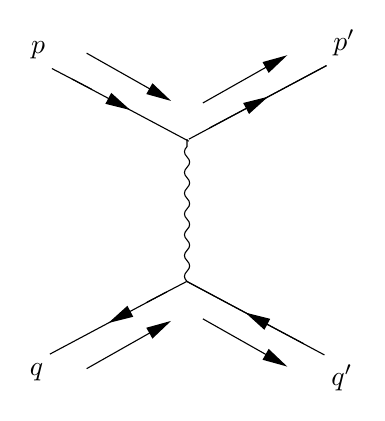
\begin{tikzpicture}[x=0.75pt,y=0.75pt,yscale=-1,xscale=1]
            %uncomment if require: \path (0,300); %set diagram left start at 0, and has height of 300
            
            %Straight Lines [id:da14290900221329284] 
            \draw    (231.69,211.94) -- (175.35,181.94) ;
            \draw [shift={(203.52,196.94)}, rotate = 28.04] [fill={rgb, 255:red, 0; green, 0; blue, 0 }  ][line width=0.08]  [draw opacity=0] (12,-3) -- (0,0) -- (12,3) -- cycle    ;
            %Straight Lines [id:da9014867833031743] 
            \draw    (175.44,181.94) -- (241.65,217.35) ;
            
            %Straight Lines [id:da009821355662845255] 
            \draw    (165.69,186.94) -- (109.35,216.94) ;
            \draw [shift={(137.52,201.94)}, rotate = 331.96] [fill={rgb, 255:red, 0; green, 0; blue, 0 }  ][line width=0.08]  [draw opacity=0] (12,-3) -- (0,0) -- (12,3) -- cycle    ;
            %Straight Lines [id:da6618699799728551] 
            \draw    (156.1,191.94) -- (175.27,181.94) ;
            
            %Straight Lines [id:da5198905686342035] 
            \draw    (175.44,181.94) .. controls (173.77,180.27) and (173.77,178.61) .. (175.44,176.94) .. controls (177.11,175.27) and (177.11,173.61) .. (175.44,171.94) .. controls (173.77,170.27) and (173.77,168.61) .. (175.44,166.94) .. controls (177.11,165.27) and (177.11,163.61) .. (175.44,161.94) .. controls (173.77,160.27) and (173.77,158.61) .. (175.44,156.94) .. controls (177.11,155.27) and (177.11,153.61) .. (175.44,151.94) .. controls (173.77,150.27) and (173.77,148.61) .. (175.44,146.94) .. controls (177.11,145.27) and (177.11,143.61) .. (175.44,141.94) .. controls (173.77,140.27) and (173.77,138.61) .. (175.44,136.94) .. controls (177.11,135.27) and (177.11,133.61) .. (175.44,131.94) .. controls (173.77,130.27) and (173.77,128.61) .. (175.44,126.94) .. controls (177.11,125.27) and (177.11,123.61) .. (175.44,121.94) .. controls (173.77,120.27) and (173.77,118.61) .. (175.44,116.94) -- (175.44,113.35) -- (175.44,113.35) ;
            %Straight Lines [id:da05547503895441053] 
            \draw    (186.31,107.94) -- (242.65,77.94) ;
            \draw [shift={(214.48,92.94)}, rotate = 151.96] [fill={rgb, 255:red, 0; green, 0; blue, 0 }  ][line width=0.08]  [draw opacity=0] (12,-3) -- (0,0) -- (12,3) -- cycle    ;
            %Straight Lines [id:da3039453718198315] 
            \draw    (242.56,77.94) -- (176.35,113.35) ;
            
            %Straight Lines [id:da5250648994964986] 
            \draw    (119.94,84.35) -- (176.27,114.35) ;
            \draw [shift={(148.1,99.35)}, rotate = 208.04] [fill={rgb, 255:red, 0; green, 0; blue, 0 }  ][line width=0.08]  [draw opacity=0] (12,-3) -- (0,0) -- (12,3) -- cycle    ;
            %Straight Lines [id:da8327140832212707] 
            \draw    (129.52,89.35) -- (110.35,79.35) ;
            
            %Straight Lines [id:da5656819062256284] 
            \draw    (127.06,223.94) -- (165.99,201.92) ;
            \draw [shift={(167.73,200.94)}, rotate = 150.51] [fill={rgb, 255:red, 0; green, 0; blue, 0 }  ][line width=0.08]  [draw opacity=0] (12,-3) -- (0,0) -- (12,3) -- cycle    ;
            %Straight Lines [id:da459463499666549] 
            \draw    (221.99,221.95) -- (183.06,199.94) ;
            \draw [shift={(223.73,222.94)}, rotate = 209.49] [fill={rgb, 255:red, 0; green, 0; blue, 0 }  ][line width=0.08]  [draw opacity=0] (12,-3) -- (0,0) -- (12,3) -- cycle    ;
            %Straight Lines [id:da5577031874748963] 
            \draw    (221.99,73.92) -- (183.06,95.94) ;
            \draw [shift={(223.73,72.94)}, rotate = 150.51] [fill={rgb, 255:red, 0; green, 0; blue, 0 }  ][line width=0.08]  [draw opacity=0] (12,-3) -- (0,0) -- (12,3) -- cycle    ;
            %Straight Lines [id:da20198354541122865] 
            \draw    (127.06,71.94) -- (165.99,93.95) ;
            \draw [shift={(167.73,94.94)}, rotate = 209.49] [fill={rgb, 255:red, 0; green, 0; blue, 0 }  ][line width=0.08]  [draw opacity=0] (12,-3) -- (0,0) -- (12,3) -- cycle    ;
            
            % Text Node
            \draw (107.35,220.34) node [anchor=north east] [inner sep=0.75pt]    {$q$};
            % Text Node
            \draw (243.65,220.75) node [anchor=north west][inner sep=0.75pt]    {$q'$};
            % Text Node
            \draw (108.35,75.95) node [anchor=south east] [inner sep=0.75pt]    {$p$};
            % Text Node
            \draw (244.65,74.54) node [anchor=south west] [inner sep=0.75pt]    {$p'$};
            \end{tikzpicture}            
    \end{gathered} \begin{aligned}[t]
        =& (-1) (- \ii e) \bar{u}(p') \gamma^\mu u(p) (- \ii e) \bar{v}(q) \gamma^\nu v(q') \frac{- \ii \eta_{\mu \nu}}{(p-p')^2 + \ii 0^+} \\
        =& - \ii e^2 \frac{1}{t} \bar{u}(p') \gamma^\mu u(p) \bar{v}(q) \gamma_\mu v(q') \eqqcolon \ii \mathcal{M}_t.
    \end{aligned}
    \label{eq:t-channel}
\end{equation}